Eräs tärkeä yhtälöiden tyyppi on \termi{potenssiyhtälö}{potenssiyhtälöt}.
\laatikko{

Potenssiyhtälö on muotoa $x^n=a$
oleva yhtälö, jossa $n$ on jokin rationaaliluku.
}

Huomaa miinus- ja murtopotenssiyhtälöissä tarkistaa, millä kantaluvuilla $x$ potenssit on määritelty. Murtopotenssia määriteltäessä vaadittiin, että kantaluku $x\geq0$
ja negatiivisen potenssin tapauksessa on huomioitava, että kantaluku $x\neq0$, sillä $x^{-a}=\frac{1}{x^a}$, eikä nimittäjässä sallita olevan lukua $0$.

Eksponentin $n$ ollessa kokonaisluku sen arvoa kutsutaan potenssiyhtälön \termi{aste (potenssiyhtälö)}{asteeksi}. Esimerkiksi potenssiyhtälön $x^2=0$ aste on $2$.

Potenssiyhtälöitä tarvitaan esimerkiksi tilanteissa, joissa lasketaan korolle korkoa.
Myös pinta-ala- ja tilavuuslaskuissa esiintyy potenssiyhtälöitä.

\laatikko{Potenssiyhtälön ratkaiseminen:
	\begin{itemize}
	\item Jos potenssiyhtälön aste $n$ on parillinen ja $a \ge 0$, yhtälöllä on kaksi ratkaisua, $$ x = \pm \sqrt[n]{a} \textrm{.} $$ ($\pm$ tarkoittaa, että sekä positiivinen että negatiivinen arvo käyvät: $\pm 5$ tarkoittaa sekä lukuja $5$ että $-5$.)
	\item Jos aste on parillinen, sillä on yksi ratkaisu vain kun $a = 0$, sillä $ x = \pm \sqrt[n]{0} = \pm 0 = 0$
	\item Jos aste on parillinen ja $a < 0$, potenssiyhtälöllä ei ole yhtään ratkaisua.
	\item Siis parillisen asteen potenssifunktiolla voi olla yksi, kaksi tai ei yhtään ratkaisua.
	\item Jos aste on pariton, ja $a \neq 0$  yhtälöllä on aina täsmälleen yksi ratkaisu, $x = \sqrt[n]{a}.$
	\item Jos aste on pariton, ja $a = 0$, yhtälöllä ei ole yhtään ratkaisua.
	\end{itemize}
}

\begin{esimerkki}
Ratkaise yhtälöt a) $x^2 = 0$, b) $x^2 - 9 = 0$ ja c) $x^2 + 9 = 0$

a)	\begin{align*}
	x^2 &= 0 \\
	x &= 0
	\end{align*}
	Yhtälöllä on yksi ratkaisu $x = 0$.

b)	\begin{align*}
	x^2 - 9 &= 0 \\
	x^2 &= 9 \\
	x &= \pm 3
	\end{align*}
	Yhtälöllä on kaksi ratkaisua $x = 3$ ja $x = -3$, sillä $3^2 = 9$ ja $(-3)^2 = 9$.

c)	\begin{align*}
	x^2 + 9 &= 0 \\
	x^2 &= -9 \\
	x &= \sqrt{-9}
	\end{align*}
	Yhtälöllä ei ole reaalista ratkaisua.

\end{esimerkki}

\laatikko{Mikäli potenssiyhtälön asteluku $n$ on pariton, yhtälöllä on aina tasan yksi ratkaisu (kun $a \neq 0$).}

\begin{esimerkki}
Ratkaise yhtälö $2x^3 + 16 = 0$

	\begin{align*}
	2x^3 + 16 &= 0 \\
	2x^3 &= -16 \\
	x^3 &= -8  \\
	x = \sqrt[3]{-8} &= -2
	\end{align*}
\end{esimerkki}

\begin{esimerkki}
	\begin{alakohdat}
		\alakohta{Yhtälö $27x^3=7$ on potenssiyhtälö, sillä jakamalla se puolittain luvulla $27$ saadaan $x^3 = \frac{7}{27}$. Tämän potenssiyhtälön aste on 3.}
		\alakohta{Yhtälö $2x^{4}-7=3$ on potenssiyhtälö, sillä se voidaan muokata muotoon $x^n = a$, ja sen aste on 4. \\
				$$2x^{4} -7 = 3$$
				$$2x^{4} = 3+7$$
				$$x^{4} = \frac{10}{2}$$
				$$x^{4} = 5.$$}
	\end{alakohdat}
\end{esimerkki}

\begin{esimerkki}
	\begin{alakohdat}
		\alakohta{Potenssiyhtälön $x^3 = 100$ ratkaisu on $x=\sqrt[3]{100}$.}
		\alakohta{Potenssiyhtälöllä $x^6 = -1$ ei ole ratkaisua, sillä $x^6 = (x^3)^2 \ge 0$ kaikilla $x$.}
		\alakohta{Potenssiyhtälöllä $x^4=50$ on kaksi ratkaisua $x=\sqrt[4]{50}=2{,}6591...$ ja $x=-\sqrt[4]{50}=-2{,}6591...$.}
	\end{alakohdat}
	\begin{center}
		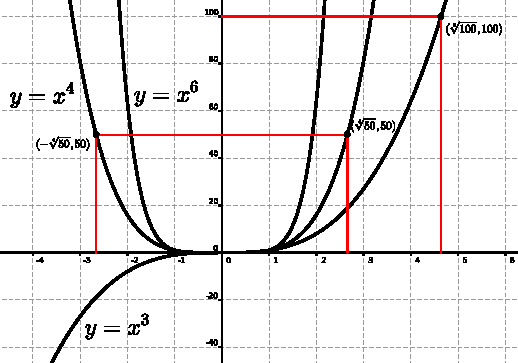
\includegraphics[width=11.5cm]{pictures/xpot346.pdf} %KUVAAJILLE ERI VÄRIT SELVENTÄISI ASIAA
	\end{center}
\end{esimerkki}

\begin{esimerkki}
Etsitään alun toisen esimerkin luku $x$, joka toteuttaa yhtälön $\frac{x^3}{3}=\frac{x^2}{2}$. Tehdään tämä kahdella tapaa vaiheittain

		\begin{align*}
			\frac{x^3}{3}&=\frac{x^2}{2} && \text{| Kerrotaan molemmat puolet kolmella.} \\
			x^3 &=\frac{3x^2}{2}   && \text{| Kerrotaan molemmat puolet kahdella.} \\
			2x^3 &=3x^2 && \text{| Vähennetään puolittain oikean puolen termillä.} \\
			2x^3 -3x^2&=0 && \text{| Jaetaan $x^2$. Huomataan ja merkitään että $x\neq0$.} \\
			%Paula Thitz: En tajua miksi yhtälön ratkaisuna ei voisi olla nolla. Olisiko selkeämpää muuttaa esim. sanamuotoon ``tarkastellaan ensin tapausta, jossa X on erisuuri kuin nolla.''
			2x -3&=0 && \text{| Lisätään molemmille puolille $3$ ja jaetaan kahdella.} \\ 
			x&=\frac{3}{2} && \\
		\end{align*}
Tutkitaan vielä erikseen tilanne $x=0$, joka ei ole määritelty yllä olevassa osamäärässä. Sijoitetaan $x=0$ yhtälöön $\frac{x^3}{3}=\frac{x^2}{2}$ ja saadaan $\frac{0^3}{3}=\frac{0^2}{2}$, joka pätee sillä $0=0$. Näin ollen siis myös $x=0$ on ratkaisu. 



Toinen tapa
\begin{align*}
\frac{x^3}{3}&=\frac{x^2}{2} && \text{| Jaetaan molemmat puolet oikean puolen termillä. } \\
\frac{x^3}{3}:\frac{x^2}{2}&=1 && \text{| Kerrotaan jakajan käänteisluvulla.} \\
\frac{x^3\cdot2}{3\cdot x^2}&=1 && \text{| Sievennetään. Huomataan ja merkitään, että nyt $x\neq0$.} \\
\frac{x\cdot2}{3}&=1 && \text{| Jaetaan puolet kahdella ja kerrotaan kolmella.} \\
x&=\frac{3}{2} && \\
\end{align*}

Tutkitaan vielä erikseen tilanne $x=0$, joka ei ole määritelty yllä olevassa osamäärässä. Sijoitetaan $x=0$ yhtälöön $\frac{x^3}{3}=\frac{x^2}{2}$ ja saadaan $\frac{0^3}{3}=\frac{0^2}{2}$, joka pätee sillä $0=0$. Näin ollen siis myös $x=0$ on ratkaisu.

Eli molemmin tavoin saatiin sama tulos, vaikka yhtälöä muokattiin eri keinoin.



\end{esimerkki}

\begin{esimerkki}
Taulutelevision kooksi (lävistäjäksi) on ilmoitettu mainoksessa $46,0$ tuumaa ($116,8$ cm) ja kuvasuhteeksi 16:9. Kuinka leveä televisio on (senttimetreinä)?

{\bf Ratkaisu.}

Taulutelevision halkaisija, alareuna ja toinen sivu muodostavat suorakulmaisen kolmion. Kolmion hypotenuusa ($c$) on television halkaisija ja kateetit ($a$ ja $b$) alareuna ja toinen sivu.

Kuvasuhteen perusteella kateettien pituuksia voidaan merkitä $16x$ ja $9x$. Pythagoraan lauseesta ($c^2 = a^2 + b^2$) saadaan
\[
(116,8)^2 = (16x)^2 + (9x)^2
\]
\[
13642,24 = (256+81)x^2.
\]
\[
x^2 = \frac{13642,24}{337}
\]
\[
x= \sqrt{\frac{13642,24}{337}} \approx 6,36.
\]
Television leveys on noin $16x = 16\cdot 6,36\approx 102$ cm.

{\bf Vastaus.} Noin $102$ cm.
\end{esimerkki}


\begin{esimerkki}
	Suursijoittaja Nalle Mursulla on $5\,000$ euroa ylimääräistä rahaa, jonka hän aikoo sijoittaa $30$ vuodeksi.  Nalle Mursu haluaa sijoittamansa pääoman kasvavan $100\,000$ euroksi $30$ vuodessa.  Kuinka suuren vuotuisen korkokannan Nalle Mursu tarvitsee sijoitukselleen? 
	\begin{esimratk}
		Olkoon vuotuinen korkokanta $r$. Korkoa korolle -periaatteen nojalla $5\,000$ euron sijoitus
		kasvaa $30$ vuodessa summaksi $5\,000\cdot(1+r)^{30}$. Merkitsemällä $x=1+r$ saamme yhtälön $5\,000\cdot x^{30} = 100\,000$.
		Jakamalla yhtälö puolittain luvulla $5\,000$ päädymme potenssiyhtälöön
		\[ x^{30} = 20, \] 
		jonka ratkaisuksi saadaan $x=20^{\frac{1}{30}} = 1{,}105\ldots$. Näin
		ollen suursijoittaja Nalle Mursun vaatima korkokanta sijoitukselleen on noin $r=1-x=1-1,105=0,105=10{,}5\,\%$.
	\end{esimratk}
\end{esimerkki}
